\documentclass[a4paper,10pt] {article}
\usepackage[top=3cm,left=3cm,right=2cm,bottom=2cm]{geometry} % definir margens da página %
\usepackage[utf8]{inputenc} % suporte a acentos %
\usepackage{graphicx} % incluir figuras %

\begin{document}

\begin {center}
UNIVERSIDADE FEDERAL DO RIO GRANDE DO SUL

Programa de Pós-Graduação em Computação - PPGC

Concepção de Circuitos VLSI - CMP115

Professor Sergio Bampi

Aluno: Daniel Munari Palomino 

\vspace{7mm}
\textbf{ TRABALHO PRÁTICO 2 - BUFFER }
\vspace{7mm}

\end{center}

\section{Objetivo}
Projetar um layout de um buffer tappered de N estágios e realizar a verificação, extração de capacitâncias parasitas a partir do layout. Além disso, realizar a caracterização elétrica do buffere gerar os seguintes resultados:

\begin{itemize}
\item Margens de ruído High e Low, obtidas a partir da função de transferência DC.
\item Valores dos tempos de resposta para o inversor projetado (Tphl, Tplh, Trise e Tfall).
\item Medir a potência consumida pelo inversor projetado à uma frequencia de chaveamento de 200MHz.
\item Calcular a energia média consumida por um par de transições L->H e H->L na saída do buffer.
\end{itemize}

\section{Projeto e Dimensionamento do Buffer}
O dimensionamento do buffer foi realizado com o objetivo de minimizar o atraso. Todo o projeto foi realizado utilizando como base o inversor projetado no trabalho 1. A figura \ref{fig:inv} apresenta o layout do inversor utilizado como base.

\begin{figure}[h]
	\label{fig:inv}
	\centering
	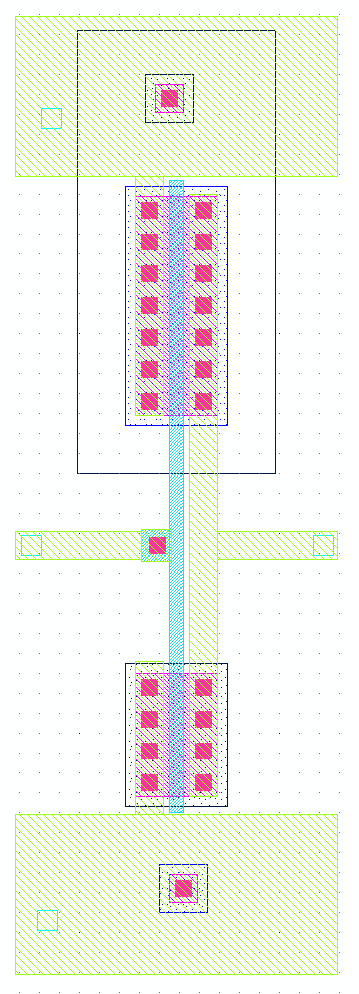
\includegraphics[scale=0.3]{layout_inversor.png}
	\caption{Layout do inversor INV\_1X}
\end{figure}

Primeiramente foi calculado o valor da capacitância de entrada Cgin, com base nas dimensões do inversor INV\_1X.

\begin{math} Cgin=(Wp+Wn).L.Cox\end{math}

\begin{math} Cgin=(5,5um+3,1um).0,35um.4,54fF\end{math}

\begin{math} Cgin=13,67fF\end{math}

Em seguida, foi realizado o cálculo do Fan-Out Efetivo.

\begin{math} F=CL/Cgin\end{math}

\begin{math} F=1pF/13,67fF\end{math}

\begin{math} F=73,15\end{math}

Com base no Fan-Out efetivo (F) foi então realizado o dimensionamento do buffer. O número de estágios foi definido visando minimizar o atraso. A tabela 1 apresenta o cálculo realizado para obtenção do número de estágios que foi utilizado no buffer. As equações utilizadas abaixo são referentes ao \begin{math} f \end{math} (fator de sizing entre os estágios) e \begin{math} tp \end{math} que é o atraso do buffer. Neste cálculo o valor de \begin{math} tp0 \end{math} foi abstraído, pois é um valor constante e o valor de gama utilizado foi igual a 1.

\begin{table}[h]
	\label{tab:table1}
	\centering
	\begin{tabular}{c|c|c}
		\hline
		\begin{math} N \end{math} & \begin{math} f=\sqrt[N]{F} \end{math} & \begin{math} tp=N.tp0.(1+f/gama) \end{math}\\
		\hline
		1 & 73,15 & 74,15 \begin{math} tp0 \end{math} \\
		2 & 8,55  & 19,1 \begin{math} tp0 \end{math} \\
		\textbf{3} & \textbf{4,12}  & \textbf {15,36 \begin{math} tp0 \end{math}} \\
		4 & 2,92  & 15,68 \begin{math} tp0 \end{math} \\
 		\hline
	\end{tabular}
	\caption{Cálculo do número de estágios para o buffer.}
\end{table}

Considerando os resultados apresentados na tabela 1, o buffer foi projetado com 3 estágios e com um fator de sizing (\begin{math} f \end{math}) igual a 4,12. Desse modo, as dimensões dos inversores que compões o buffer foram as seguintes:

\begin{itemize}
\item INV\_1: \begin{math} Wp=5,5um \end{math} e \begin{math} Wn=3,1um \end{math}
\item INV\_2: \begin{math} Wp=22,0um \end{math} e \begin{math} Wn=12,4um \end{math}
\item INV\_3: \begin{math} Wp=88,0um \end{math} e \begin{math} Wn=49,6um \end{math}
\end{itemize}

A figura \ref{fig:buffer} apresenta o layout do buffer considerando os cálculos apresentados anteriormente. A técnica de \textit{foldding} foi utilizada para possibilitar o layout do buffer no espaço determinado na especificação do trabalho (altura da célula, 20um).

\begin{figure} [h]
	\label{fig:buffer}
	\centering
	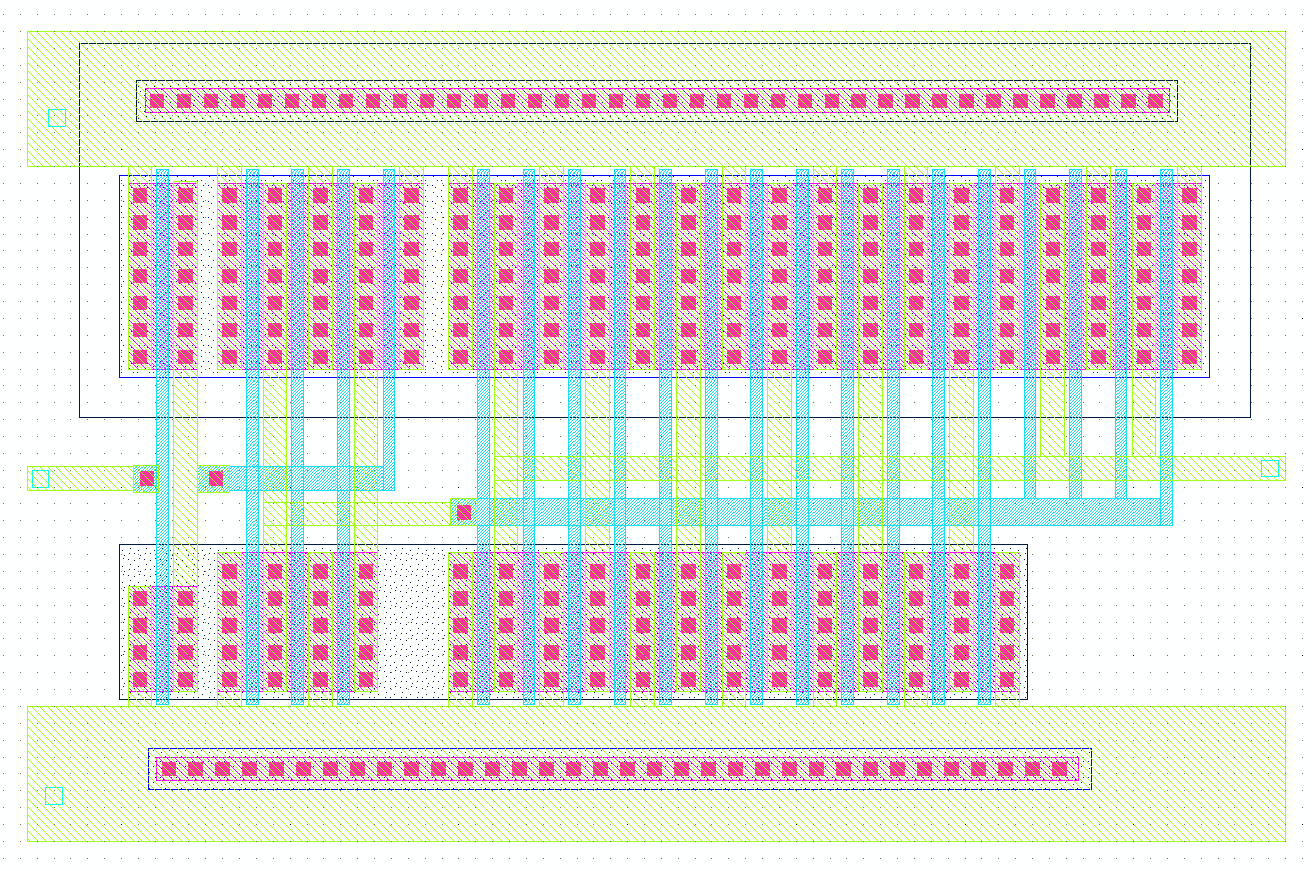
\includegraphics[scale=0.25]{layout_buffer.png}
	\caption{Layout do buffer projetado}
\end{figure}

\section{Verificações}
\label{sec:veri}
A primeira verficação realizada sobre o projeto do layout do buffer foi a verficação DRC. A figura \ref{fig:drc} apresenta a saída do software para a verficação DRC. É possível observar que nenhum erro foi encontrado.

\begin{figure} [h]
	\label{fig:drc}
	\centering
	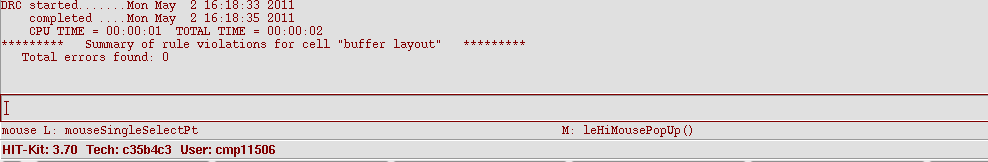
\includegraphics[scale=0.15]{DRC_buffer.png}
	\caption{Resultado verficação DRC.}
\end{figure}

O esquemático do buffer também foi construído, afim de realizar a verificação LVS (\textit{layout versus squematic}). A figura \ref{fig:esquematico} apresenta o esquemático referente ao buffer projetado e a figura \ref{fig:lvs} apresenta o resultado da verificação LVS.

\begin{figure} [h]
	\label{fig:esquematico}
	\centering
	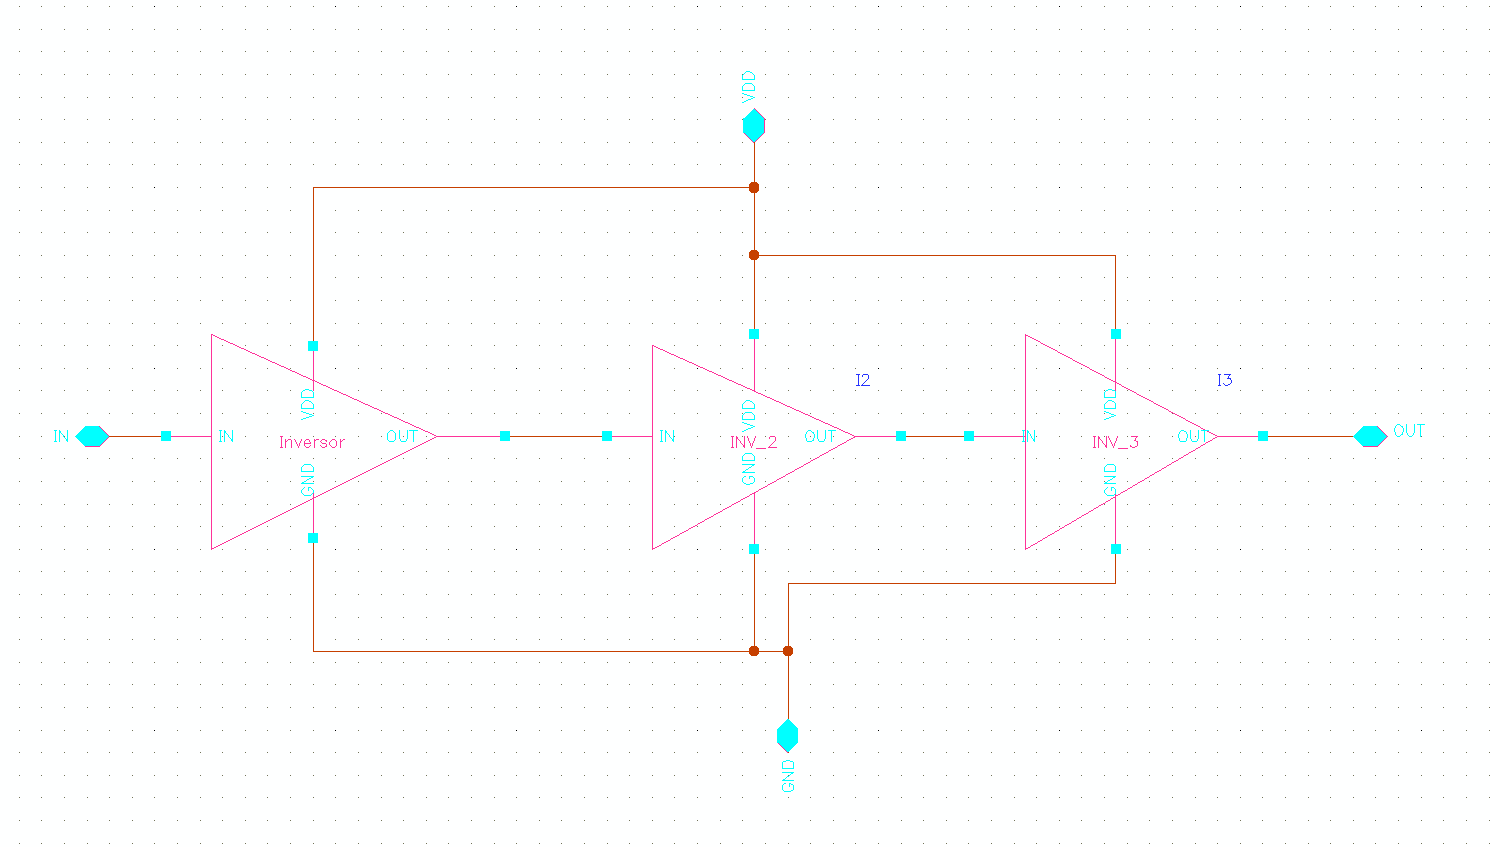
\includegraphics[scale=0.15]{esquematico_buffer.png}
	\caption{Esquemático do buffer projetado.}
\end{figure}

\begin{figure} [h]
	\label{fig:lvs}
	\centering
	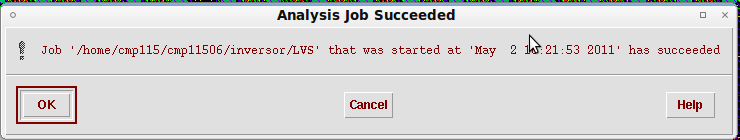
\includegraphics[scale=0.1]{LVS_buffer.png}
	\caption{Resultado da verificação LVS.}
\end{figure}

A extração das capacitâncias parasitas também foi realizada. O layout com as capacitância parasitas extraídas foi utilizado para realizar a caracterização elétrica do buffer projetado, que será apresentada na próxima seção. A figura \ref{fig:extraido} apresenta o layout do buffer com as capacitâncias parasitas extraídas.

\begin{figure} [h]
	\label{fig:extraido}
	\centering
	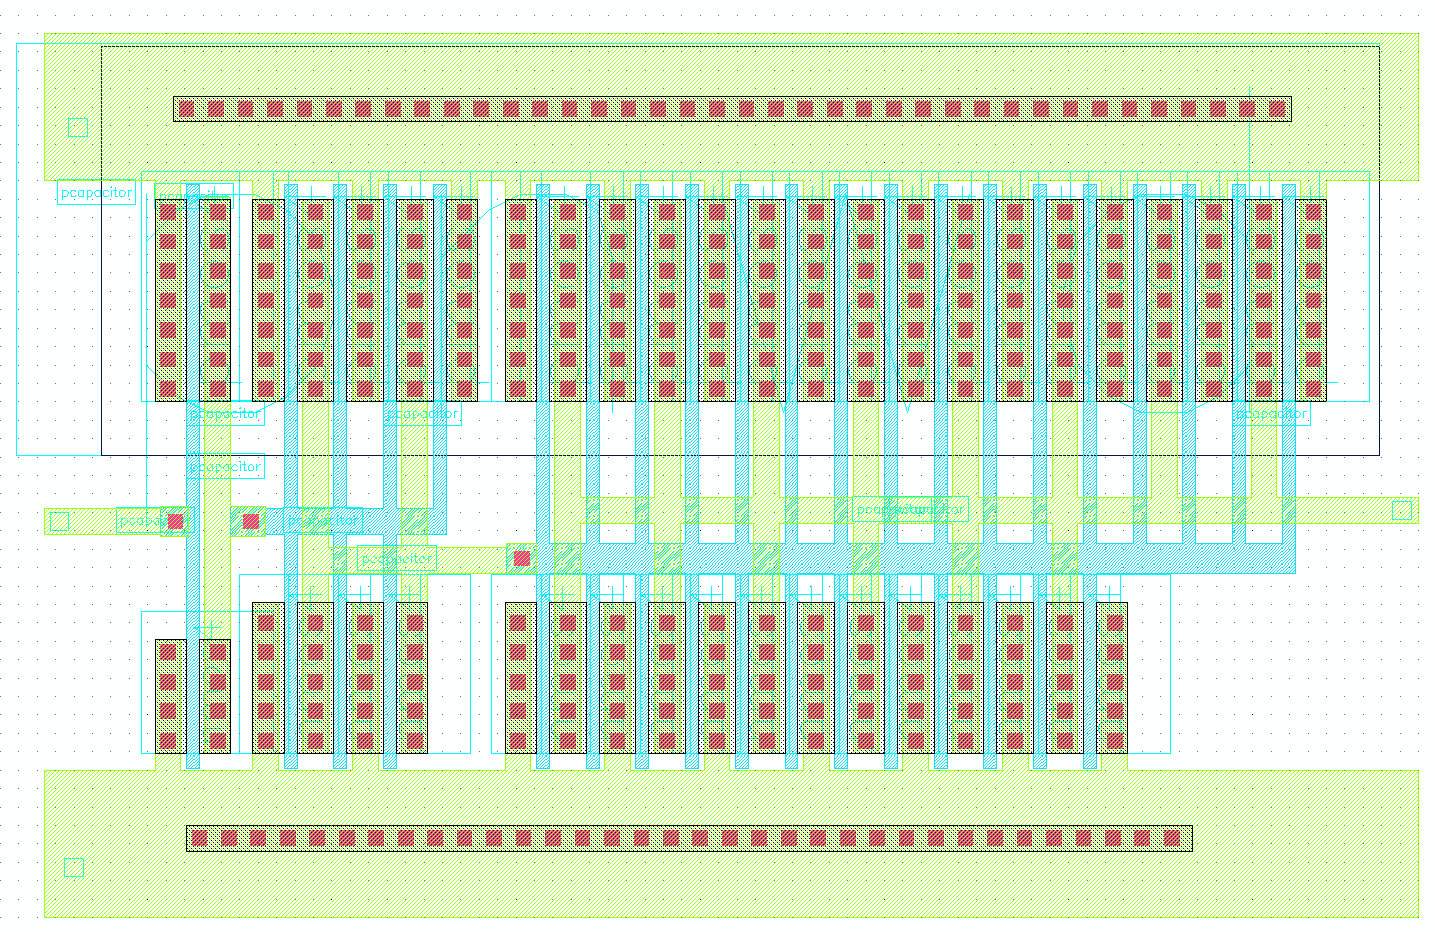
\includegraphics[scale=0.2]{extraido_buffer.png}
	\caption{Layout do buffer projetado com as capacitâncias parasitas extraídas.}
\end{figure}

\section{Caracterização Elétrica}
\label{sec:caracterizacao}
O modelo de simulação utilizado está representado na figura \ref{fig:teste}. A fonte vdc na entrada foi utilizada para obter a curva de transferência DC enquanto que a fonte vpulse foi utilizada para realizar a ánalise transiente. A carga utilizada na saída é de $1pF$, como descrito na especificação.

\begin{figure} [h]
	\label{fig:teste}
	\centering
	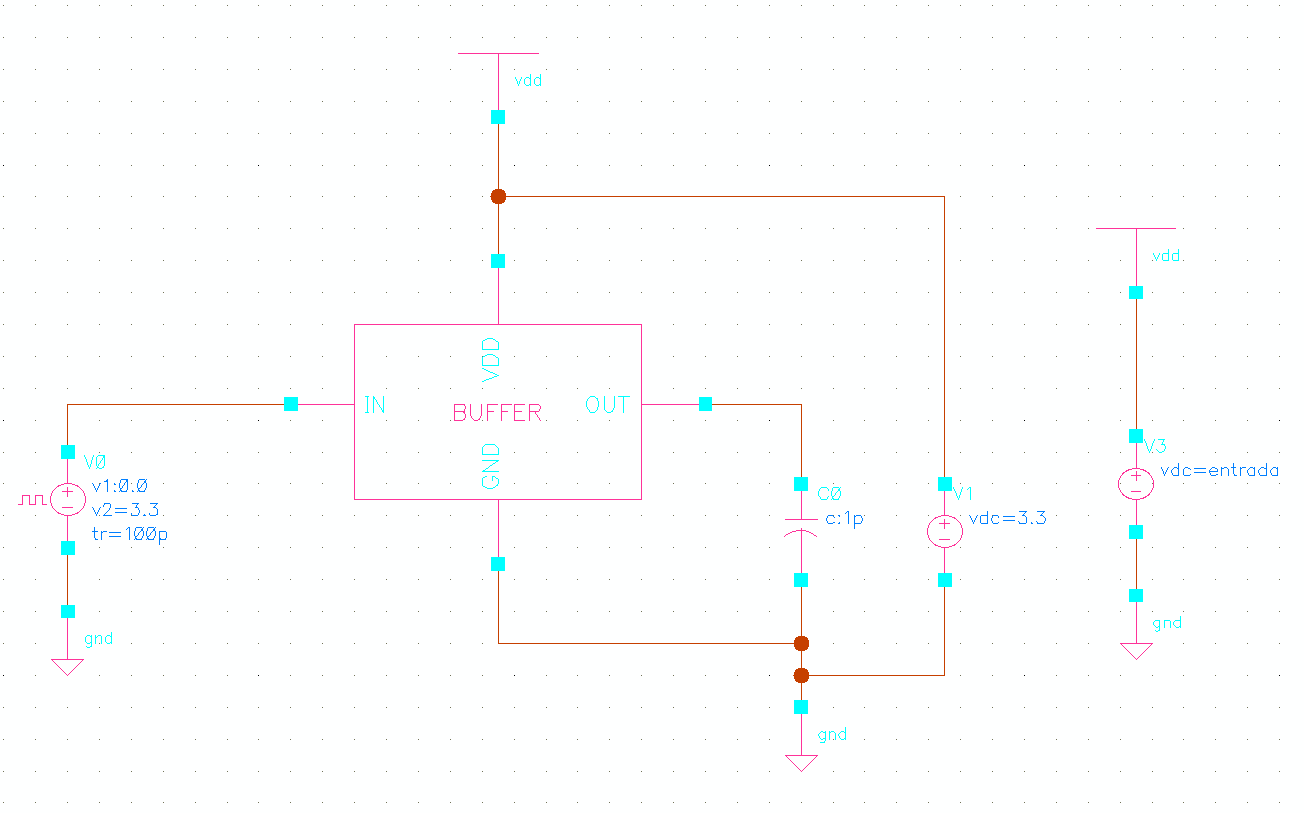
\includegraphics[scale=0.15]{teste_buffer.png}
	\caption{Modelo de simulação utilizado para realizar a caracterização elétrica do buffer.}
\end{figure}

Primeiramente foi gerada a função de transferência DC para o cálculo das margens de ruído High e Low. A figura \ref{fig:dc} apresenta a curva que representa função de transferência DC onde os pontos marcaados são referentes aos limites das margens de ruído.

\begin{figure} [h]
	\label{fig:dc}
	\centering
	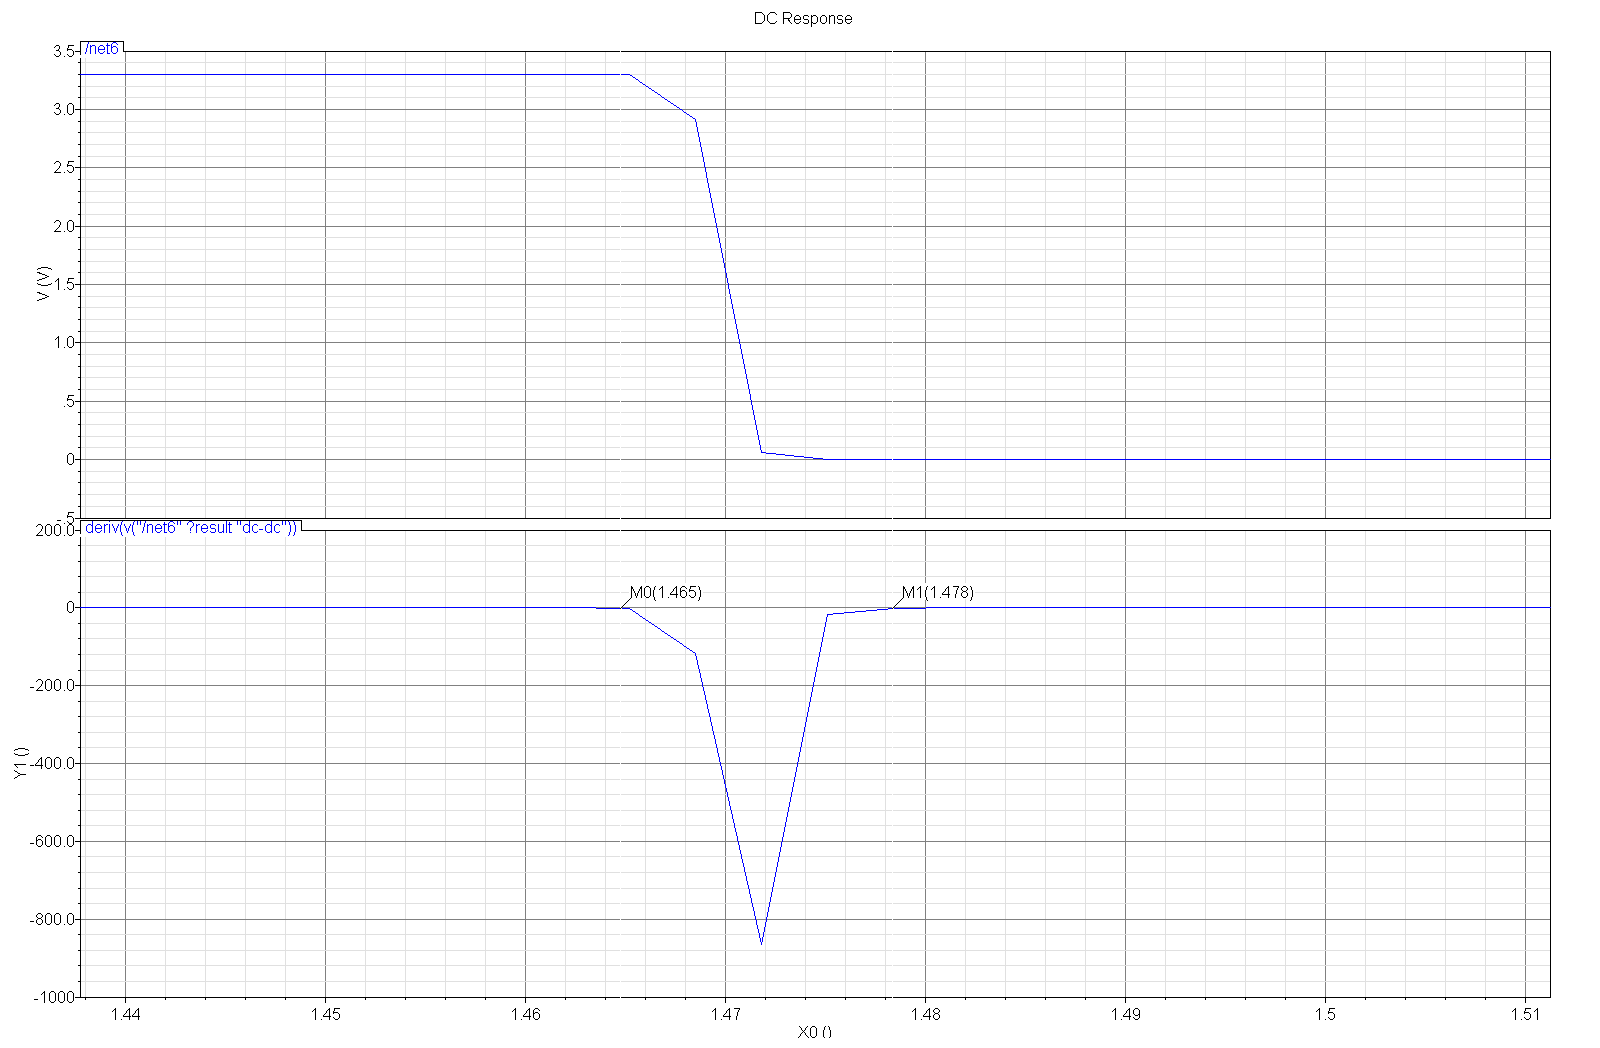
\includegraphics[scale=0.1]{DC_Buffer.png}
	\caption{Curva de transferência DC.}
\end{figure}

Desse modo, a margem de ruído Low é 0V à 1.465V e a margem de ruiído High é 1.478V à 3.3V.

Considerando a ánalise transiente quatro tempos de resposta foram medidos: (1)Tphl, (2)Tplh, (3)Trise e (4)Tfall. As figuras \ref{fig:hl}, \ref{fig:lh}, \ref{fig:rise} e \ref{fig:fall} mostram como esses tempos foram obtidos.

\begin{figure} [h]
	\begin{minipage} [b] {0.48 \linewidth}
		\fbox{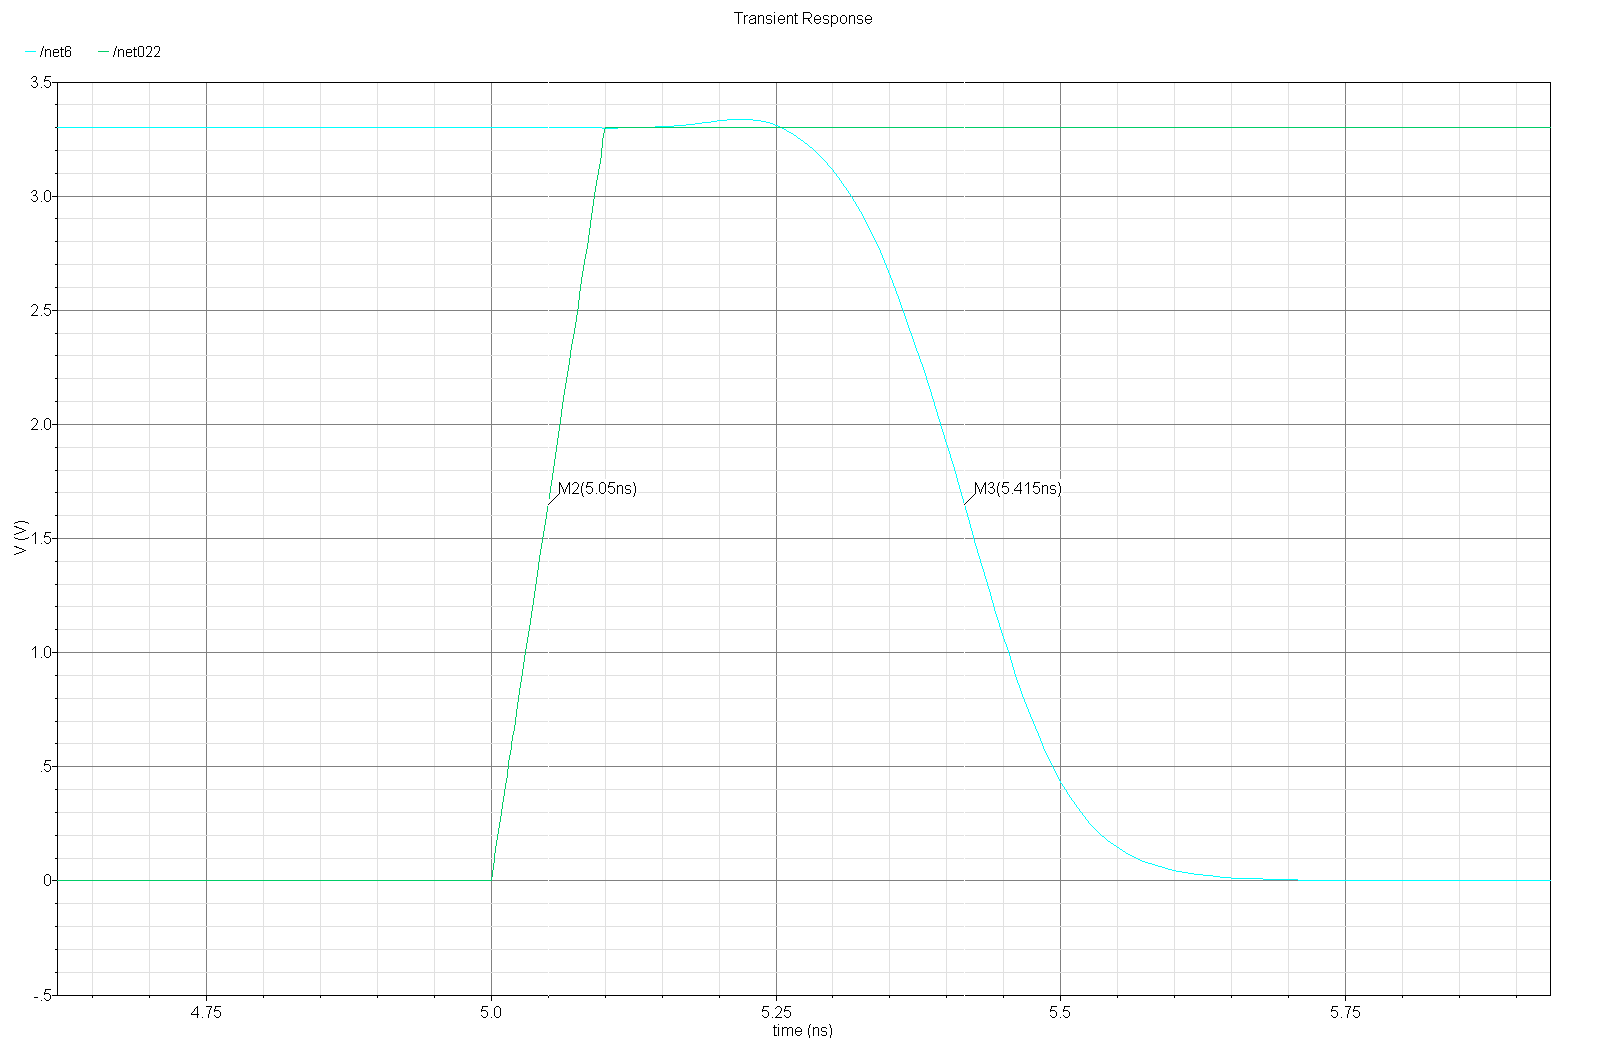
\includegraphics[scale=0.1]{Trans_HL.png}}\\
		\label{fig:hl}
		\centering
		\caption{Curva de tempo High Low.}
	\end{minipage}
	\begin{minipage} [b] {0.48 \linewidth}
		\fbox{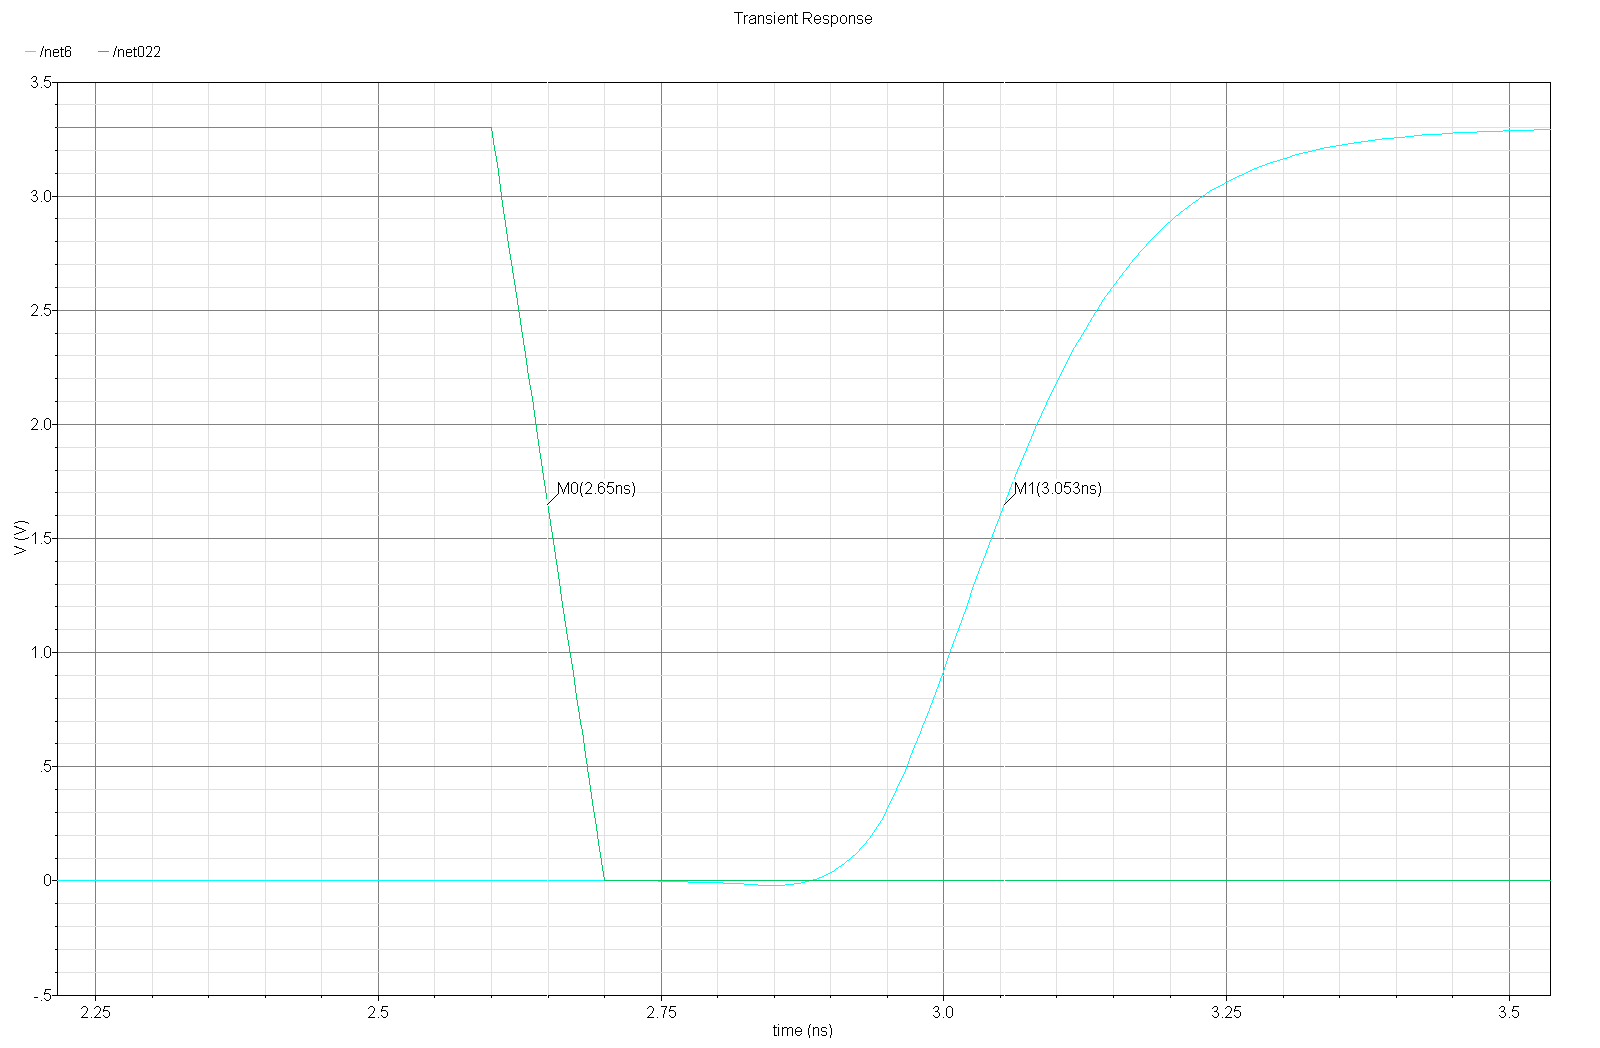
\includegraphics[scale=0.1]{Trans_LH.png}}\\
		\label{fig:lh}
		\centering
		\caption{Curva de tempo Low High.}
	\end{minipage}
\end{figure}

\begin{figure} [h]
	\begin{minipage} [b] {0.48 \linewidth}
		\fbox{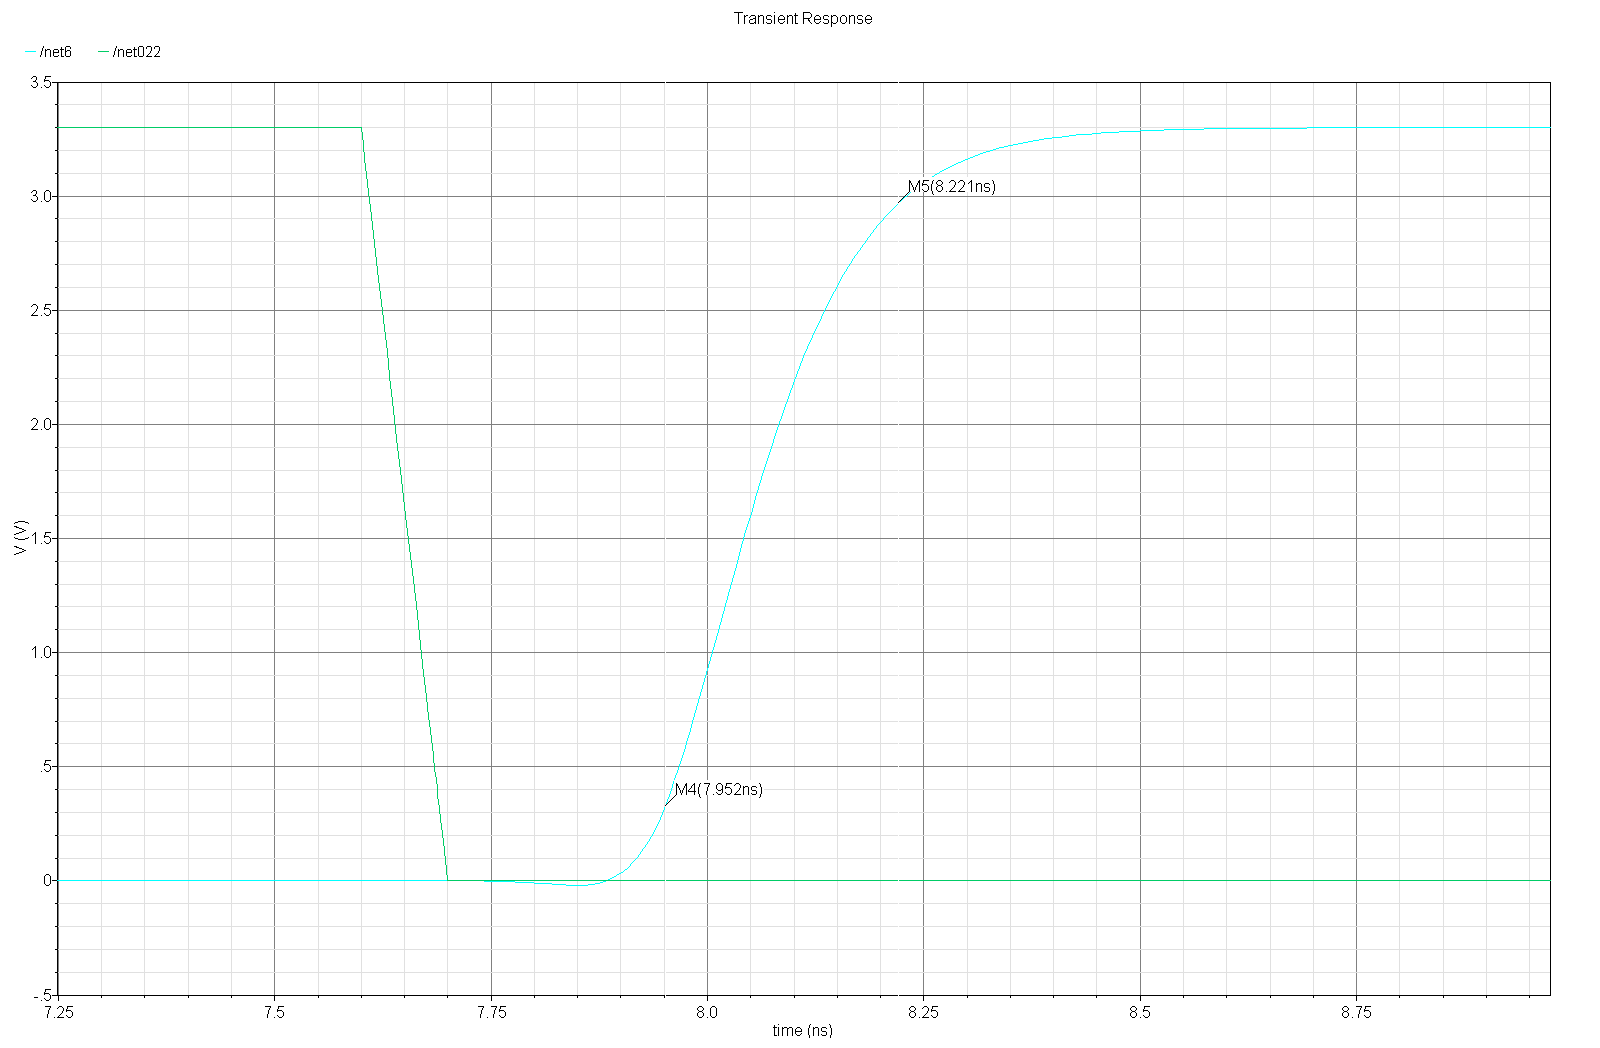
\includegraphics[scale=0.1]{Trans_rise.png}}
		\label{fig:rise}
		\centering
		\caption{Curva de tempo de subida.}
	\end{minipage}
	\begin{minipage} [b] {0.48 \linewidth}
		\fbox{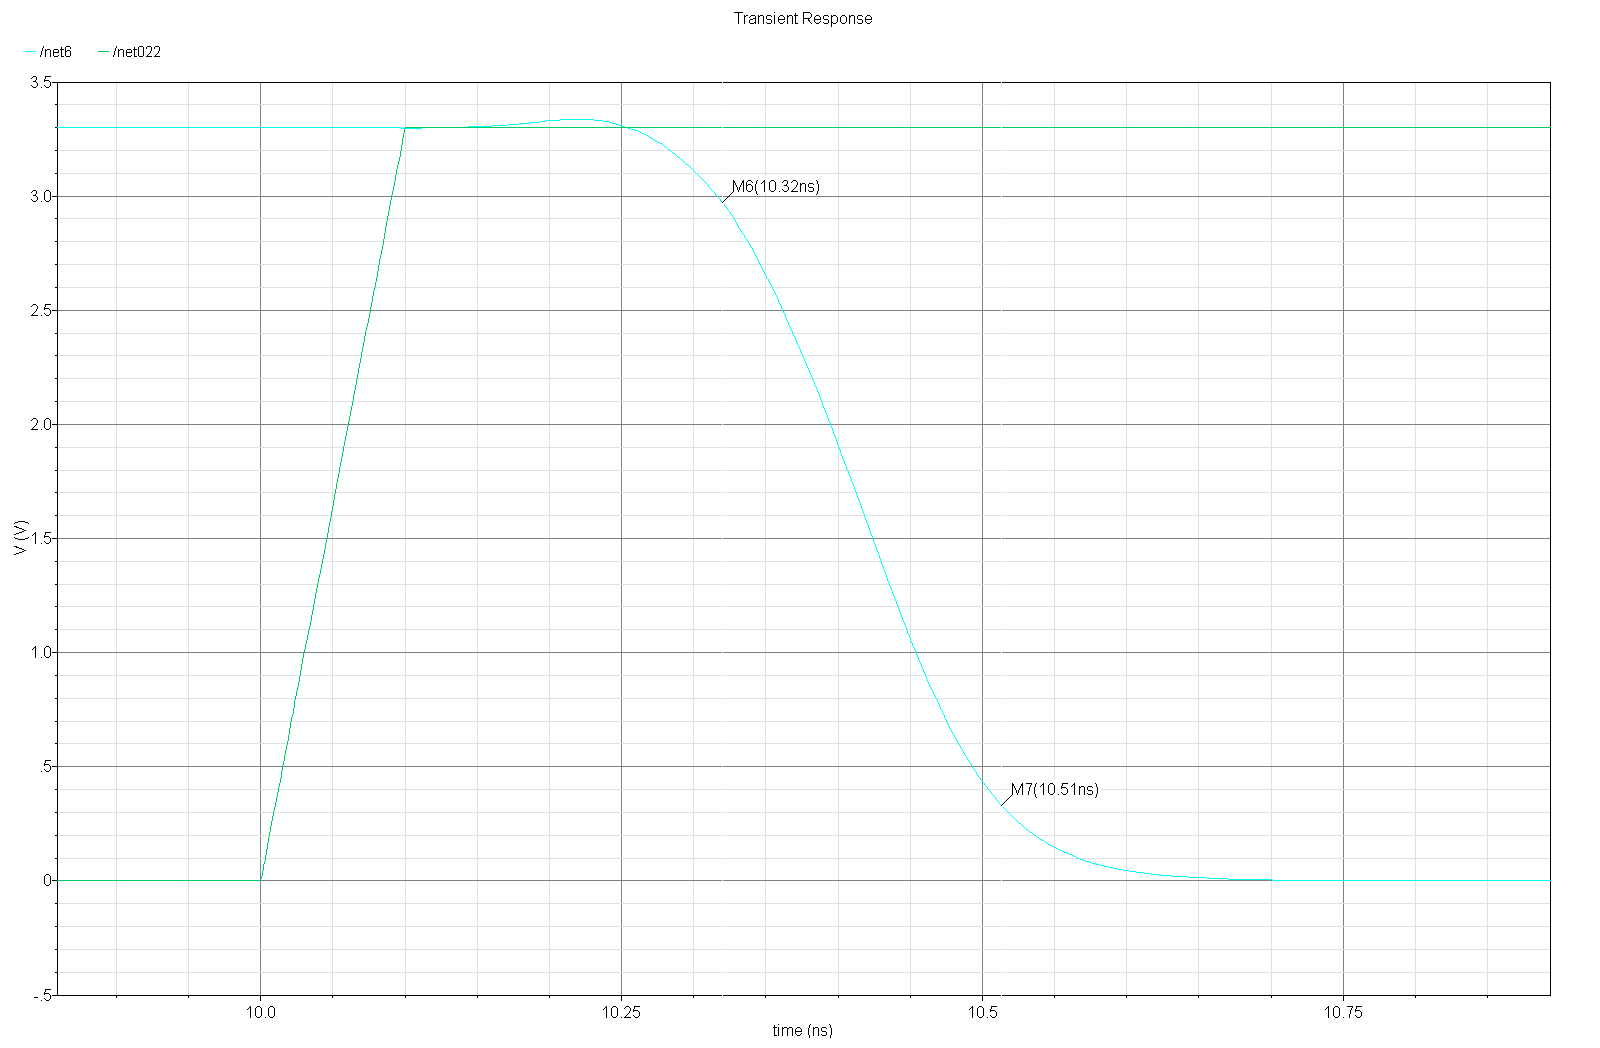
\includegraphics[scale=0.1]{Trans_fall.png}}
		\label{fig:fall}
		\centering
		\caption{Curva de tempo de descida.}
	\end{minipage}
\end{figure}

Com base nas curvas apresentadas acima, os tempos de resposta para o buffer projetado foram os seguintes:

\begin{itemize}
\item $Tphl=M3-M2=5,415ns-5,050ns=0.365ns$
\item $Tplh=M1-M0=3,053ns-2,650ns=0.403ns$
\item $Trise=M5-M4=8,221ns-7,952ns=0,269ns$
\item $Tfall=M7-M6=10,51ns-10,32ns=0,19ns$
\end{itemize}

O passo seguinte foi realizar a medição da potência consumida pelo buffer projetado. O modelo de simulação mostrado na figura x também foi utilizado nesta etapa. A frequência de chaveamento utilizada foi de 200MHz. A figura x mostar a curva que representa a corrente de alimentação utilizada no cálculo da potência.

\begin{figure} [h]
	\label{fig:corrente}
	\centering
	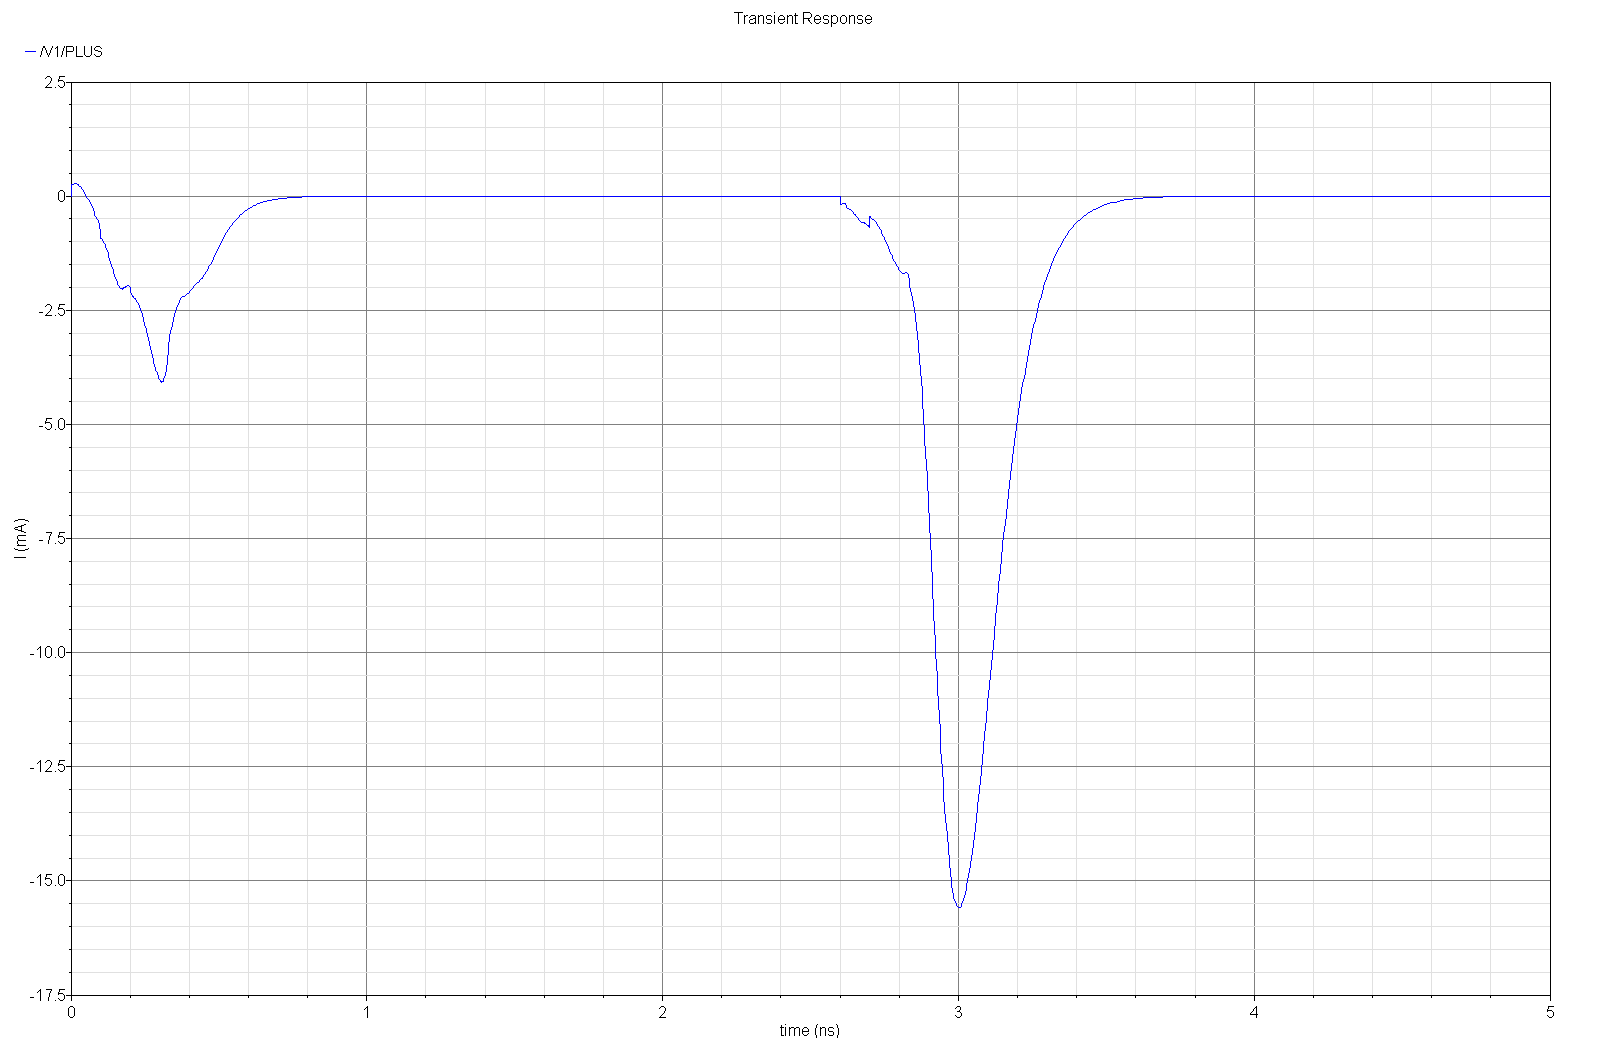
\includegraphics[scale=0.1]{Corrente.png}
	\caption{Curva de tempo de descida.}
\end{figure}

A potência consumida pelo inversor foi de 3,511mW. Sendo assim, a energia consumida por uma par de transições L->H e H->L na saída do inversor foi de 17,6pJ.

\section{Referências}




\end{document}
